\chapter{Raccolta e analisi dei requisiti}
	\section{Descrizione della realtà di interesse}
	L'idea è stata quella di creare una gestione delle code senza essere presenti fisicamente, in modo da sfruttare il proprio tempo in maniera più efficiente.
	Quante volte è capitato di stare in fila alla posta o dal medico? Persino ad un ricevimento di un professore. Tante. Il tempo è una delle poche risorse che l'essere umano non è in grado di riclare.
	
	\textbf{L'obbiettivo che ci siamo posti come team è di creare una piattaforma user-friendly, utile e accessibile}.
	Chiunque può iscriversi e creare una stanza a cui gli altri iscritti possono partecipare, chattare, o scambiare posti in coda. 
	\section{Funzionalità offerte}
	Le funzionalità offerte dall'applicazione sono molteplici e mirate a raggiungere gli scopi sopracitati. Ogni visitatore può iscriversi utilizzando la propria mail, attivando il proprio account tramite un link inviato via posta, oppure attraverso i più famosi social network come \textbf{Google} o \textbf{Facebook}.
	
	Ogni iscritto avrà a propria disposizione una sezione profilo con all'interno un avatar, il contatore delle partecipazioni, un id hashato e un link che consente di invitare visitari in modo da guadagnare punti.
	
	Si può creare una stanza inserendo nome, descrizione, numero partecipanti e facoltativamente luogo. Il tutto può essere pubblico o privato, nella seconda alternativa si può accedere soltanto se si conosce il link della stanza.
	
	Si ricompensano gli utenti che mantengono la loro promessa di frequentazione assegnandogli punti, esperienza e aumentando il loro contatore nella sezione profilo. Ovviamente è presente una sezione leaderboard che contiente la classifica globale del sito.
	
	Le stanze possono essere ricercate tramite la barra di ricerca oppure trovandole nella mappa: per posizione personale oppure tramite località. Non è possibile, ovviamente, prenotarsi per stanze piene ma, è possibile tramite messaggi privati, richiedere lo scambio posizione con chi è già in attesa.
	
	Il sito prevede anche un servizio di messaggistica, come sopra citato, che può essere usato per chattare normalmente o per richiedere posti nelle code delle stanze che ci interessano.
	
	\subsection{Sign-up e sign-in}
	\label{sec:signup}
	Nel sito si ha la possibilità di scegliere: essere un \textbf{guest} o \textbf{user}. Da ruoli diversi, derivano differenti poteri. Un guest ha la possibilità di vedere room e ricercarle tramite località, può controllare le code di un stanza ma, non può partecipare. La musica cambia nel caso in ci si autentica. Un utente ha tutti i poteri del guest e in più può creare room e partecipare, mandare messaggi e vedere la leaderboard.
	
	La registrazione può essere effettuata tramite email, con password scelta dall'utente, oppure attraverso \textbf{Oauth} con i più famosi servizi: Google e Facebook. Nel caso si scelga la prima alternativa, il sistema genererà una mail di conferma che sarà inviata all'indirizzo immesso. Questa procedura non è necessaria nel caso si utilizzi l'oauth.
	
	%US da 1 a 5%
	\begin{figure}[H]
		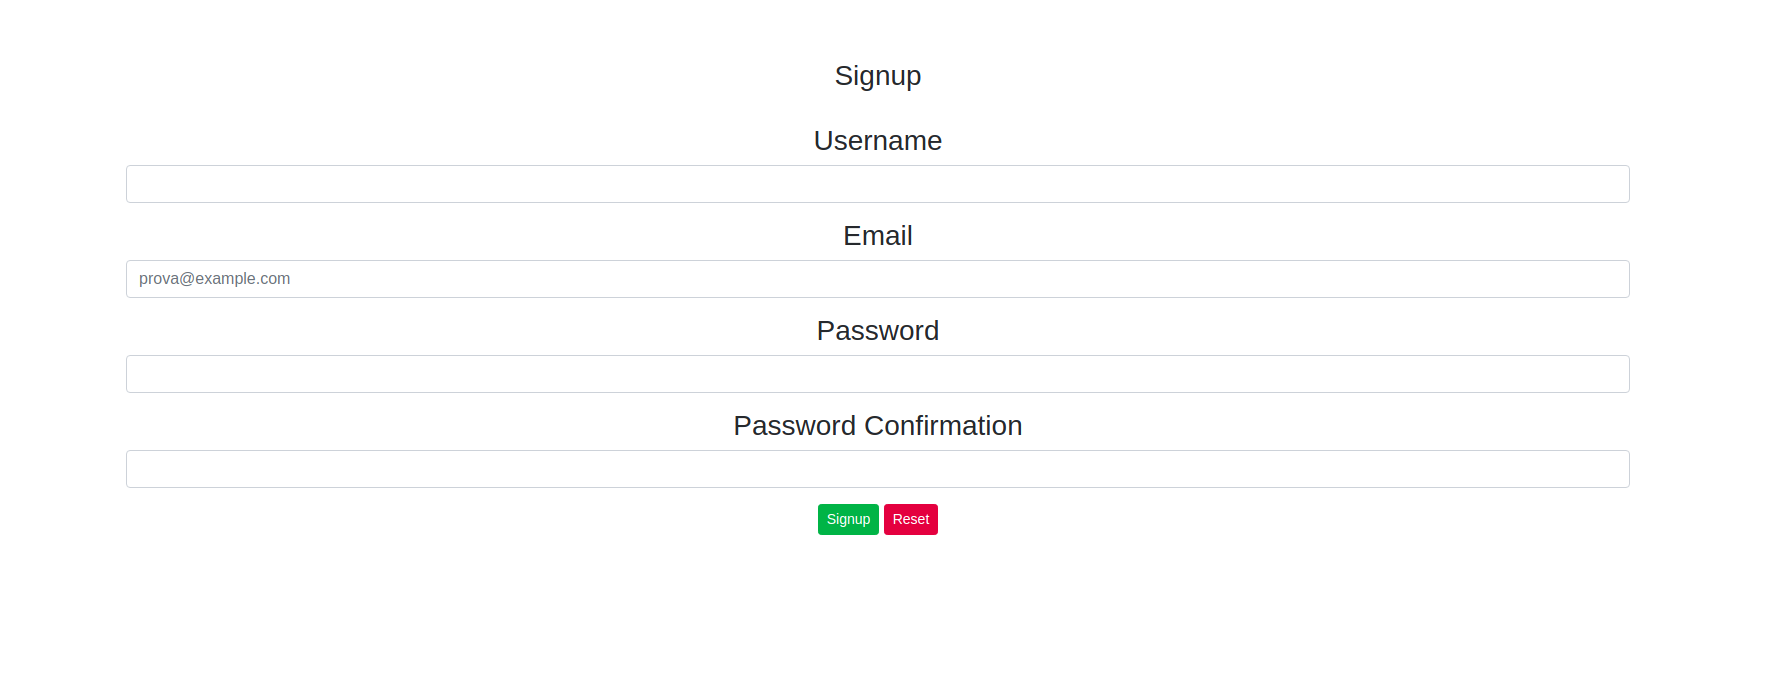
\includegraphics[width=\columnwidth]{./media/image11.png}
		\caption{Schermata sign up}
	\end{figure}	
	Le user-stories relative a questa sezione sono:\\\
	\texttt{1.As an UNREGISTERED USER i want to SIGN UP WITH MY EMAIL so \\ that i can BECOME A USER}\\
	\texttt{2.As an UNREGISTERED USER i want to SIGN UP WITH MY FACEBOOK OR \\ GMAIL ACCOUNT so that i can BECOME A USER}\\\
	
	Per un utente già registrato ma senza una sessione attiva si ha la possibilità di effettuare il sign-in.
	\begin{figure}[H]
		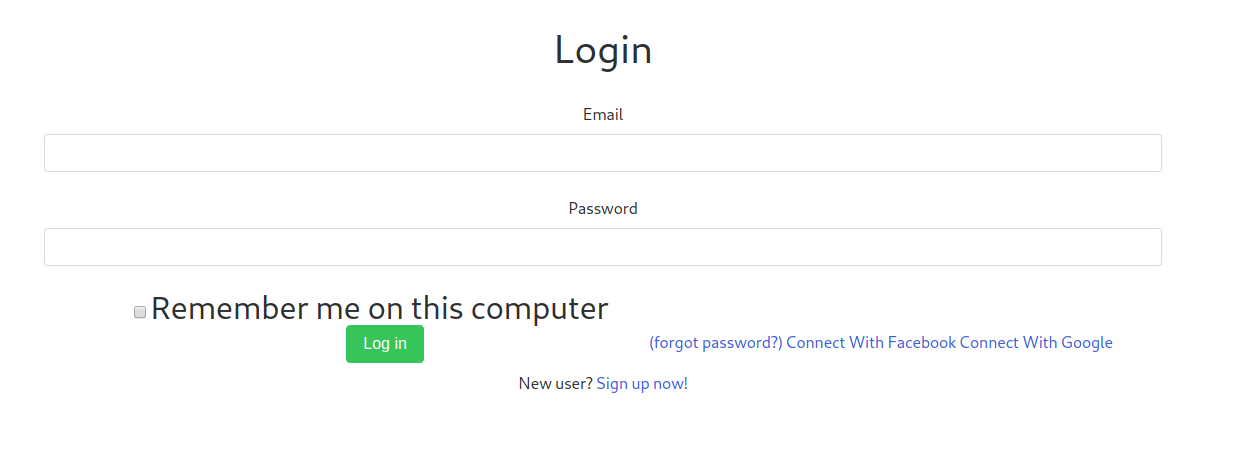
\includegraphics[width=\columnwidth]{./media/image9.png}
		\caption{Schermata sign in}
	\end{figure}
	Le user-stories relative a questa porzione sono:\\
	\texttt{3. As a USER i want to LOG IN WITH MY EMAIL so that i can \\ ACCESS THE WEBSITE}\\
	\texttt{4. As a USER i want to LOG IN WITH MY FACEBOOK OR GMAIL ACCOUNT \\ so that i can}\\
	
	E' possibile, in caso di smarrimento, chiedere il reset della password. Verrà inviata una mail contenente un link che rimanda alla apposita sezione.
	\begin{figure}[H]
		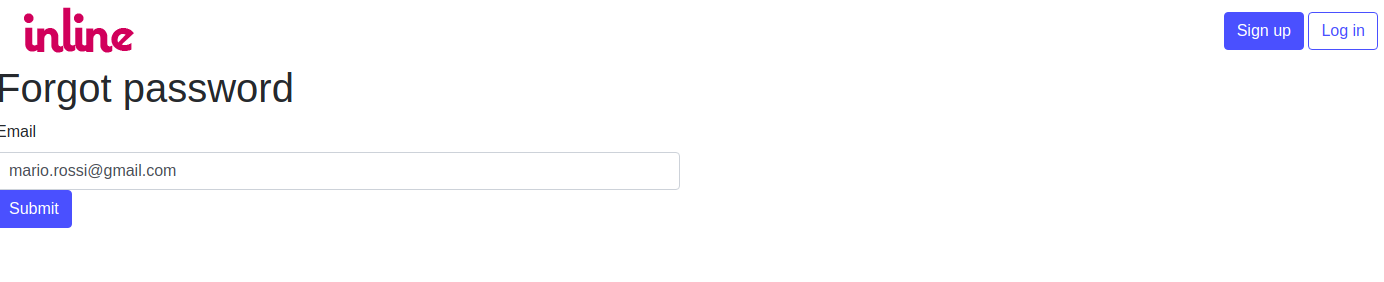
\includegraphics[width=\columnwidth]{./media/image7.png}
		\caption{Schermata reset password smarrita}
	\end{figure}
	
		La user-story relativa a questa sezione sono:\\
	\texttt{5.As a USER i want to GENERATE A LINK TO MODIFY MY PASSWORD so \\ that i can RECOVER MY PASSWORD}\\\\

	\subsection{Profilo}
	E' presente una sezione profilo personale, che contiene tutti i dati immessi nella fase di registrazione. Nella fase di \hyperref[sec:signup]{sign-up} non è richiesto immettere dati reali eccetto per l'email, salvaguardando quindi la privacy dell'utente.\\\\
	Si è scelto di rendere l'id utente un hash per una maggiore sicurezza: non è così possibile scorrere gli utenti del sito in maniera cronologica ma soprattutto, non è possibile individuare gli admin, caso banale in ci fossero stati gli id numerici.\\\\
	Con il referal link è possibile invitare conoscenti ad iscriversi, guadagnando così punti nella leaderboard. All'invitato arriverà una mail con il referal link dell'utente invitante.\\\\
	\begin{figure}[H]
		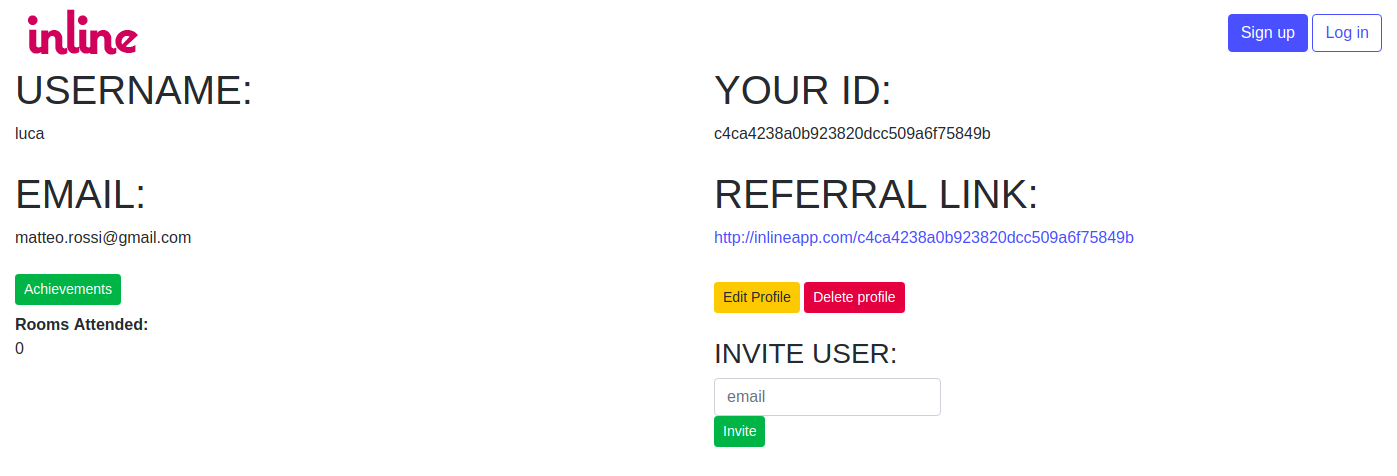
\includegraphics[width=\columnwidth]{./media/image14.png}
		\caption{Schermata profilo}
	\end{figure}
	La user-story relativa a questa sezione sono:\\
	\texttt{6. As a USER i want to SHARE MY REFERRAL LINK so that i can \\ INVITE MY FRIENDS AND INCREASE MY RANK}\\
		
	E' possibile modificare i propri dati all'interno del sito, in modo da mantenere aggiornati con la realtà. Si può cambiare e-mail, password e per i casi più estremi si ha la possibilità di eliminare ogni traccia del proprio account sul sito.
	
	La user-story relativa a questa sezione sono:\\
	\texttt{7. As a USER i want to HAVE SETTINGS so that i can UPDATE MY \\ PROFILE}\\
	\texttt{8. As a USER i want to HAVE SETTINGS so that i can CHANGE MY \\ PASSWORD}\\
	\texttt{9. As a USER i want to HAVE SETTINGS so that i can DELETE MY \\ PROFILE}\\
	\\
	Porzione collegata al referal link è la leadeboard, che tiene traccia delle stanze a cui hai partecipato o che hanno riscosso tanto successo, fornendo esperienza. I modi per ottenere punti sono i seguenti:
	\begin{itemize}	
		\item Invitare amici tramite l'apposito input nel profilo.
		\item Partecipare ad una stanza, con successiva verifica.
		\item Una stanza creata da te ha riscosso un notevole successo.
	\end{itemize}

	\begin{figure}[H]
		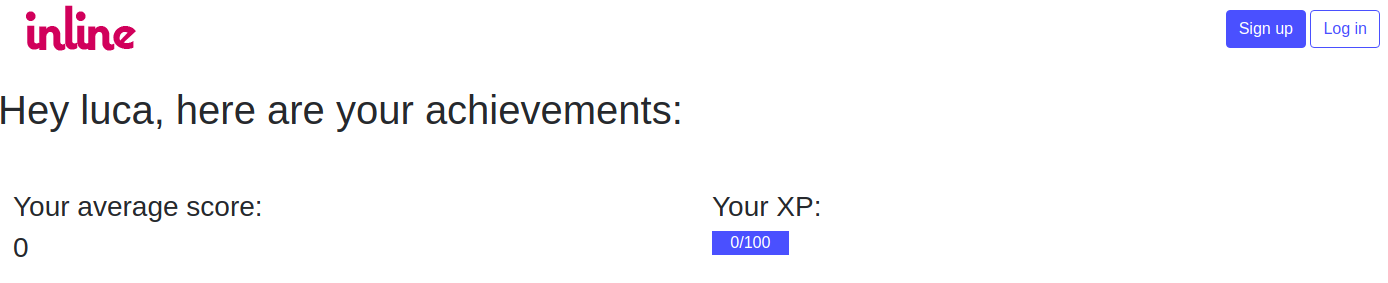
\includegraphics[width=\columnwidth]{./media/image6.png}
		\caption{Schermata achievements}
	\end{figure}

	La user-story relativa a questa sezione sono:\\\\
	\texttt{12. As a USER i want to HAVE ACHIEVEMENTS so that i can SEE MY \\ RATING}\\
	\texttt{13. As a USER i want to HAVE ACHIEVEMENTS so that i can SEE HOW \\ MANY ROOMS I ATTENDED}\\
	\texttt{14. As a USER i want to HAVE ACHIEVEMENTS so that i can SEE MY \\ RANK}

	\subsection{Room}
	
	\subsubsection{Creazione}
	Le stanze sono il cuore pulsante del progetto, possono essere create da tutti coloro che sono registrati, quindi anche admin. Una room può essere creata tramite il bottone nella toolbar, inserendo nome, descrizione, ora e data. Le rooms che riscuotono successo genereranno esperienza per i room host collegati. 
	
	Le room private, rese tali dalla decisione del proprietario, non compaiono nella homepage, barra di ricerca oppure mappa. L'unico modo di accere è tramite invito o link. Dopo la sottoscrizione ad una stanza nascosta l'utente è in grado di vederla normalmente.
	
	E' possibile ricercare una località a cui la room fa riferimento tramite l'api di \textbf{mapbox} compilando l'apposito input, in caso di località non presente è consigliato aggiungerla nella descrizione. La ricorrenza delle stanze è un'idea che è stata resa possibile tramite un gem \textit{recurring-select}, che permette di iterare un evento ogni porzione di tempo che si vuole. Per comodità sono state inserite nel sito le più usate: \textit{Every day, every week, every month, every year}.
	
	I radio buttons in alto segnalo l'opzione di scegliere il tipo di coda, argomentata nella prossima sottosezione, che può essere una fifo o una priority queue.
	\begin{figure}[H]
		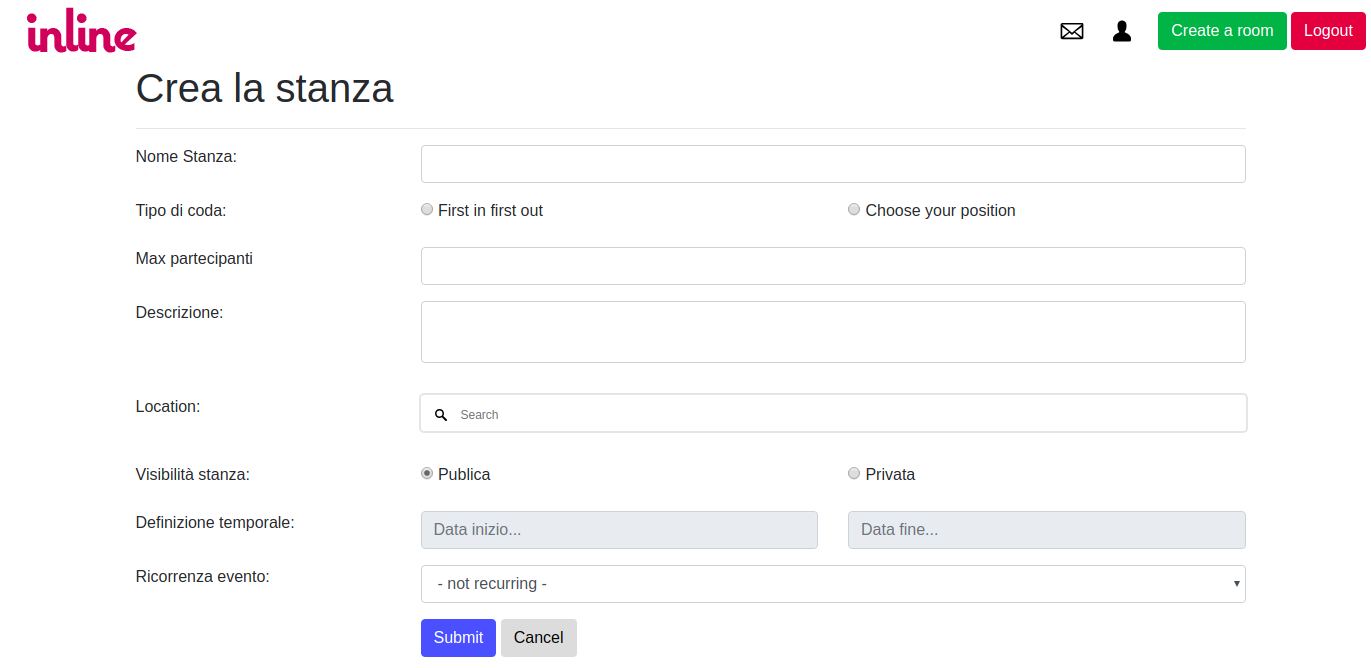
\includegraphics[width=\columnwidth]{./media/image8.png}
		\caption{Creazione stanza}
	\end{figure}
	La user-story relativa a questa sezione sono:\\
	\texttt{18. As a ROOM HOST i want to USE MAPBOX so that i can PIN AN \\ ADDRESS ON A MAP}\\
	\texttt{19. As a USER i want to USE GOOGLE CALENDAR so that i can SEE \\ INCOMING EVENTS}\\
	\texttt{20. As a ROOM HOST i want to USE GOOGLE CALENDAR so that i can \\ TRACK AND SET RECURRENT EVENTS}\\\\
	

	\subsubsection{Gestione coda}
	Essendo una parte core, abbiamo deciso di impostare la coda secondo due metodologie differenti, basandoci su due strutture dati ben note nel mondo informatico. \textbf{FIFO}, first-in-first-out, e la \textbf{Priority queue}, erano le due migliori alternative candidate a risolvere questo problema. 
	
	Nella prima soluzione, la più semplice poi da implementare, è soltanto necessario scegliere di partecipare alla stanza, il sistema farà il restante. E' possibile, tramite la visione della coda, capire approssimativamente il momento del proprio turno. Nel caso in cui l'antecedente cancelli la propria prenotazione, viene rimosso dalla queue facendo avanzare i successori.
	
	La seconda scelta, invece, si differenzia dalla prima per poter scegliere il proprio slot in modo da poter assecondare le proprie necessità. Questo tipo di coda è più consigliata ad incontri con medici, professori o persino alla posta.
	
	Entrambe le opzioni prevedono la possibilità di scambio, avanzata, tramite messaggio privato cliccando l'icona accanto al proprio nickname nella coda. L'utente verrà reindirizzato nella pagina dei messaggi privati, come oggetto verrà utilizzato il seguente template \textbf{[utenteRichiedente NomeStanza in DateTime swapRequest from PosNum to PosNum]}. 
	
	Il destinatario riceverà una proposta che potrà rifiutare o accettare tramite pulsanti presente nella comunicazione.\\
	
	La user-story relativa a questa sezione sono:\\
	\texttt{26. As a USER i want to JOIN A ROOM so that i can RESERVE A SPOT}\\
	\texttt{27. As a USER i want to UNJOIN A ROOM so that i can CANCEL MY \\ RESERVATION}\\
	\texttt{28. As a USER i want to REQUEST ANOTHER USER'S SPOT IN THE QUEUE so that i can SWITCH MY POSITION}\\
	\texttt{29. As a USER i want to REPORT A ROOM OR USER so that i CAN \\ ALERT AN ADMIN}
	
	\subsubsection{User side}
	L'utente, una volta effettuata la sottoscrizione alla stanza ha a disposizione la chat associata room che consente di restare in contatto con gli organizzatori, in caso di imprevisti, o di comunicare con gli altri partecipanti. L'utente non può in nessun effettuare azioni di \textit{delete} o \textit{update} dei messaggi. Questo compito spetta rigorosamente ai moderatori e ai room-hosts.
	
	In caso di scorrettezze è possibile segnalare qualsiasi cosa ad un admin del sito, che accoglierà la segnalazione e verificherà di conseguenza.
	
	Alla sinistra della schermata si può notare la mappa con relativo pin sulla posizione esatta dell'evento, nel caso in cui la mappa non fosse presente è perché il room host ha preferito non dare un indirizzo fisico alla stanza. Due input ineditabili alla sinistra mostrano la data e ora dell'evento.
	
	E' possibile utilizzare \textbf{Google Calendar} per tenere traccia delle proprie sottoscrizioni, infatti troviamo un link che aggiunge un evento al calendario personale. Il codice verrà esaminato nei capitoli successivi, per ora ci limitiamo a listare le varie features.
	
	Quando un evento è imminente, si riceverà un email che ricorderà data, ora e luogo se presente della stanza a cui ci si è sottoscritti.
	
	\begin{figure}[H]
		\includegraphics[width=\columnwidth]{roomPQ.png}
		\caption{Room con priority queue vista da un utente}
	\end{figure}

	\subsection{Room host side}
	Appena creata la stanza un messaggio flash, ci avviserà della corretta fondazione. Un room-host avrà poteri amministrativi relativi solo alle room che creato o alla quale è stato nominato tale da altri room-hosts.
	
	I messaggi della chat presentano una croce rossa e una matita in alto a destra costruendo, in questo modo, un sistema di moderazione a cui partecipano solo gli utenti con poteri.
	
	Nonostante si hanno tutti i poteri necessari per far funzionare al meglio la stanza, un room-host non potrà \textit{mai e poi mai}: cambiare, cancellare o creare prenotazioni.
	
	Nella parte alta della pagina è presente un input che offre la funzionalità di invitare utenti nella stanza, questo funziona sia se la room è pubblica o privata. Appena sotto è presente un link che cliccando, ci reindirizzerà nella pagina di edit, consentendoci di modificare i principali campi.
	
	In caso di presenza, che essa sia fisica o virtuale, l'host della room provvederà a votare l'utente, con un pollice al fianco della prenotazione della persona interessata.
	\begin{figure}[H]
		\includegraphics[width=\columnwidth]{room.png}
		\caption{Room vista da un room host}
	\end{figure}

	\begin{figure}[H]
		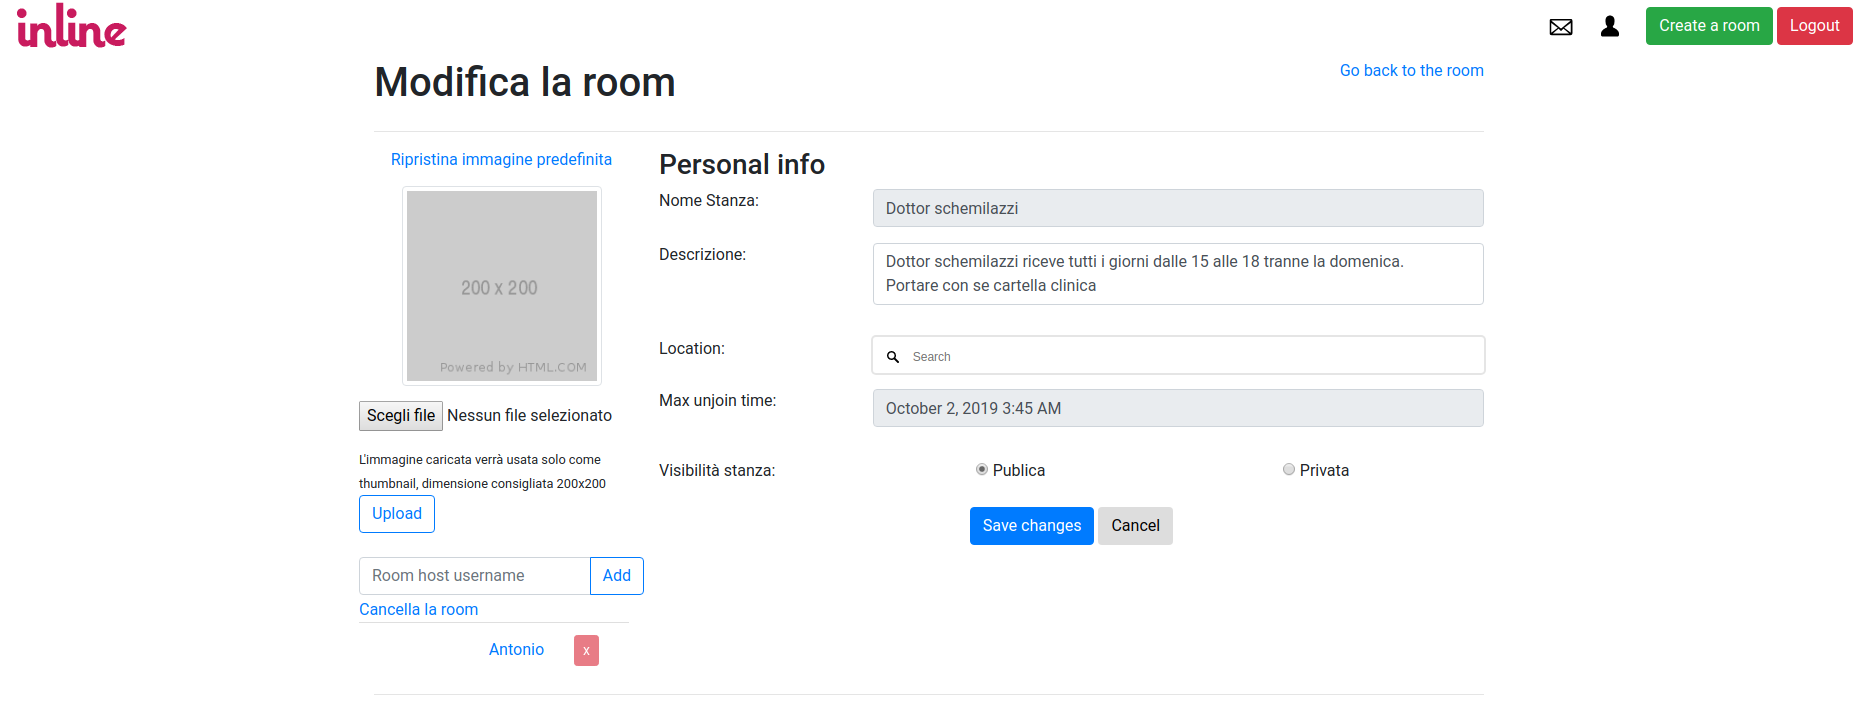
\includegraphics[width=\columnwidth]{./media/EditRoom.png}
		\caption{vista dell'edit room}
	\end{figure}

	Le user stories relative a queste due sottosezioni sono:\\
	\texttt{21. As a USER i want to HAVE A CHAT IN THE ROOM so that i can\\ COMMUNICATE WITH OTHER ROOM PARTICIPANTS}\\
	\texttt{22. As a ROOM HOST i want to HAVE SPECIAL PRIVILEGES so that i \\ can EDIT MESSAGES}\\
	\texttt{23. As a ROOM HOST i want to HAVE SPECIAL PRIVILEGES so that i \\ can PIN A MESSAGE}\\
	\texttt{25. As a USER i want to BE NOTIFIED OF MY INCOMING EVENT so \\ that i can HAVE A REMINDER SENT VIA EMAIL}\\
	\texttt{30. As a ROOM HOST i want to HAVE SPECIAL SETTINGS so that i \\ can EDIT A ROOM’S PARAMETERS}\\
	\texttt{31. As a ROOM HOST i want PROMOTE ANOTHER USER TO ROOM HOST to \\ so that HE CAN HAVE HOST PRIVILEGES}\\
	\texttt{32. As ROOM HOST i want to CHECK THE EVENT ATTENDEES so that i \\ can RATE A USER}\\
	\texttt{33. As ROOM HOST i want to INVITE USERS TO MY ROOM so that i \\ can ALERT THEM OF THE EVENT}
	
	\section{Dashboard}
	Una persona, che sia registrata o un visitatore, riesce a vedere la dashboard, che comprende le principali funzioni di ricerca e listing delle room.
	
	Si presenta con una mappa in alto, contentente, tutte le stanze vicino alla propria posizione o, occasionalmente, si può ricercare, tramite la barra di ricerca, le room per nome e per raggio o per località.
	Le stanze che vengono ricercate compariranno sulla mappa, di conseguenza, scompariranno quelle che non corrispondono alla query.
	
	Vicino alla barra è presente un pulsante che consente di centrare la propria posizione sulla mappa, fornendo le opportune autorizzazioni al browser.
	
	Le room sono listate al di sotto della mappa in un riquadro per ciascuna che contiene descrizione, luogo, un link per visitare la stanza e, al passaggio del mouse, rivelerà i room hosts.
	
	\begin{figure}[H]
		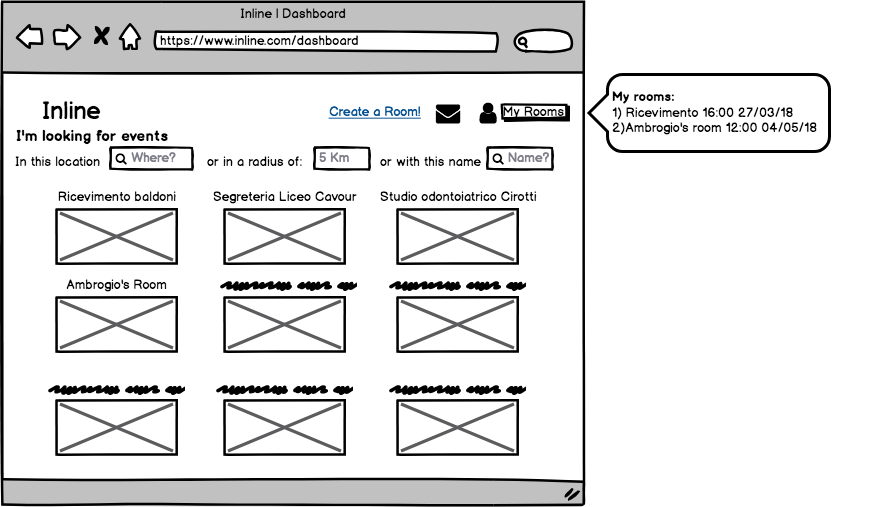
\includegraphics[width=\columnwidth]{./media/dashboard.png}
		\caption{Vista della dashboard}
	\end{figure}

	Le user stories relative a questa sezione sono:\\
	\texttt{15. As a USER i want to USE MAPBOX so that i can SEE WHERE THE \\ EVENT IS LOCATED ON A MAP}\\
	\texttt{16. As a USER i want to USE MAPBOX so that i can SEE ROOMS IN A \\ DETERMINED RADIUS NEAR ME}\\
	\texttt{17. As a USER i want to USE MAPBOX so that i can SEE ROOMS IN A \\ CERTAIN LOCATION}\\
	\texttt{24. As a USER i want to USE THE SEARCH BAR so that i can \\ FIND ROOMS}\\
	\texttt{34. As an UNREGISTERED USER / USER i want to USE THE DASHBOARD\\ so that i can SEE PUBLICLY LISTED ROOMS}\\
	\texttt{35. As a USER i want to SEE THE ROOMS I’M CURRENTLY ATTENDING \\ so that i can KEEP TRACK OF THEM}\\
	
	\section{Messaggi privati}
	E' stato concesso agli utenti la possibilità di interagire tra di loro al di fuori delle room, tutto grazie ai messaggi privati. 
	In una qualsiasi pagina del sito è possibile cliccare sull'icona della posta e creare un DM per un qualsiasi utente iscritto.
	
	La schermata presenta tre input diversi:
	\begin{itemize}
		\item Destinatario, un qualsiasi utente iscritto al sito, a patto che abbia l'opzione di ricevere messaggi privati attivata.
		\item Oggetto, un titolo per l'argomento del messaggio.
		\item Testo, il corpo del messaggio o l'invito a scambiare un posto alla coda.
	\end{itemize}
	\begin{figure}[H]
		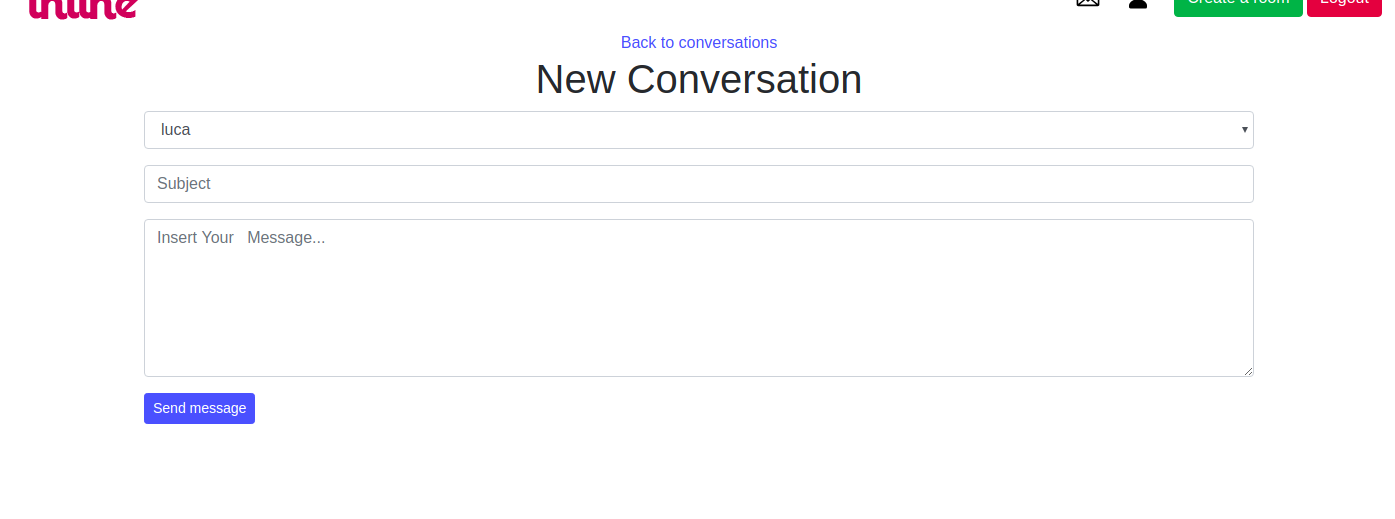
\includegraphics[width=\columnwidth]{./media/image10.png}
		\caption{Vista dei messaggi privati}
	\end{figure}

	\section{Admin}
	Ogni sito che si rispetti ha una persona a comando che gestisce e controlla gli iscritti o semplicimente modifica i contenuti.
	Nel nostro caso un admin ha la possibilità di cancellare ogni traccia di un utente oppure bannarlo, a seconda dall'azione scorretta compiuta.
	
	E' presente una dashboard accessibile solo da admin o utenti eletti da essi. Si ha accesso a tutte le funzioni sopracitate e in più si può sospendere il sito, per manutenzione o motivi tecnici.
	
	L'admin ha il potere di cambiare la maggior parte dei parametri all'interno della piattaforma come, ad esempio, quelli delle room, se violano le politiche del sito oppure campi utenti per gli stessi motivi. 
	
	L'amministratore riesce a vedere tutte le stanze presenti, in modo da favorire il proprio compito di moderazione.\\\\
	
	\begin{figure}[H]
		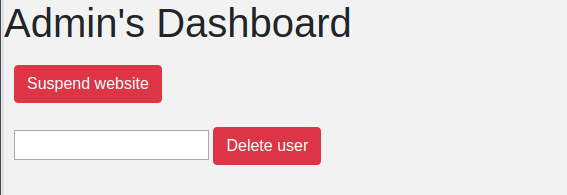
\includegraphics[width=\columnwidth]{./media/image2.png}
		\caption{Vista della dashboard admin}
	\end{figure}

	Le user stories relative a questa sezione sono:\\
	\texttt{36. As an ADMIN i want to HAVE SPECIAL SETTINGS so that i can \\ DELETE A USER}\\
	\texttt{37. As an ADMIN i want to HAVE SPECIAL SETTINGS so that i can \\ HANDLE A USER’S STATUS}\\
	\texttt{38. As an ADMIN i want to HAVE SPECIAL PRIVILEGES so that i can \\ SEE ALL ROOMS}\\
	\texttt{39. As an ADMIN i want to HAVE SPECIAL SETTINGS so that i can \\ SUSPEND THE WEBSITE}\\
	\texttt{40. As an ADMIN i want to HAVE SPECIAL PRIVILEGES so that i can \\ MODIFY ANY ROOM}\\
	
	\section{User stories}
	Per la progettazione del sito abbiamo usato le user stories che, un linguaggio informale per descrivere le features della piattaforma dal punto di vista dell'end user, il tutto piò essere paragonato a dei post-it. Per chiarezza esporremo le user storie raggruppate nelle sezioni appena affrontate.
	
	\subsection{Sezione utente e profilo}
	\texttt{1. As an UNREGISTERED USER i want to SIGN UP WITH MY EMAIL so \\ that i can BECOME A USER}\\
	\texttt{2. As an UNREGISTERED USER i want to SIGN UP WITH MY FACEBOOK \\ OR GMAIL ACCOUNT so that i can BECOME A USER}\\
	\texttt{3. As a USER i want to LOG IN WITH MY EMAIL so that i can ACCESS THE WEBSITE}\\
	\texttt{4. As a USER i want to LOG IN WITH MY FACEBOOK OR GMAIL ACCOUNT \\so that i can}\\
	
	\subsection{Sezione accesso al sito web}
	\texttt{5. As a USER i want to GENERATE A LINK TO MODIFY MY PASSWORD so \\ that i can RECOVER MY PASSWORD}\\
	\texttt{6. As a USER i want to SHARE MY REFERRAL LINK so that i can \\ INVITE MY FRIENDS AND INCREASE MY RANK}\\
	\texttt{7. As a USER i want to HAVE SETTINGS so that i can UPDATE MY \\ PROFILE}\\
	\texttt{8. As a USER i want to HAVE SETTINGS so that i can CHANGE MY \\ PASSWORD}\\
	\texttt{9. As a USER i want to HAVE SETTINGS so that i can DELETE MY \\ PROFILE}
	
	\subsection{Sezione messaggi privati}
	\texttt{10. As a USER i want to HAVE PRIVATE MESSAGES so that i can \\ MESSAGE ANOTHER USER}\\
	\texttt{11. As a USER i want to HAVE PRIVATE MESSAGES so that i can \\ RECEIVE MESSAGES FROM OTHER USERS}
	
	\subsection{Sezione achievements}
	
	\texttt{12. As a USER i want to HAVE ACHIEVEMENTS so that i can SEE \\ MY RATING}\\
	\texttt{13. As a USER i want to HAVE ACHIEVEMENTS so that i can SEE \\ HOW MANY ROOMS I ATTENDED}\\
	\texttt{14. As a USER i want to HAVE ACHIEVEMENTS so that i can SEE\\  MY RANK}
	
	\subsection{Sezione servizi esterni}
	\texttt{15. As a USER i want to USE MAPBOX so that i can SEE WHERE THE \\ EVENT IS LOCATED ON A MAP}\\
	\texttt{16. As a USER i want to USE MAPBOX so that i can SEE ROOMS IN A \\ DETERMINED RADIUS NEAR ME}\\
	\texttt{17. As a USER i want to USE MAPBOX so that i can SEE ROOMS IN A \\ CERTAIN LOCATION}\\
	\texttt{18. As a ROOM HOST i want to USE MAPBOX so that i can PIN AN \\ ADDRESS ON A MAP}\\
	\texttt{19. As a USER i want to USE GOOGLE CALENDAR so that i can SEE \\ INCOMING EVENTS}\\
	\texttt{20. As a ROOM HOST i want to USE GOOGLE CALENDAR so that i can \\ TRACK AND SET RECURRENT EVENTS}
	
	
	\subsection{Sezione chat}
	\texttt{21. As a USER i want to HAVE A CHAT IN THE ROOM so that i can \\ COMMUNICATE WITH OTHER ROOM PARTICIPANTS}\\
	\texttt{22. As a ROOM HOST i want to HAVE SPECIAL PRIVILEGES so that i \\ can EDIT MESSAGES}\\
	\texttt{23. As a ROOM HOST i want to HAVE SPECIAL PRIVILEGES so that i \\ can PIN A MESSAGE}
	
	\subsection{Sezione ricerca}
	\texttt{24. As a USER i want to USE THE SEARCH BAR so that i can FIND \\ ROOMS}
	
	\subsection{Sezione notifica}
	
	\texttt{25. As a USER i want to BE NOTIFIED OF MY INCOMING EVENT so \\ that i can HAVE A REMINDER SENT VIA EMAIL}
	
	\subsection{Sezione room}
	
	\texttt{26. As a USER i want to JOIN A ROOM so that i can RESERVE A \\ SPOT}\\
	\texttt{27. As a USER i want to UNJOIN A ROOM so that i can CANCEL MY\\  RESERVATION}\\
	\texttt{28. As a USER i want to REQUEST ANOTHER USER'S SPOT IN THE \\ QUEUE so that i can SWITCH MY POSITION}\\
	\texttt{29. As a USER i want to REPORT A ROOM OR USER so that i CAN \\ ALERT AN ADMIN}\\
	\texttt{30. As a ROOM HOST i want to HAVE SPECIAL SETTINGS so that i \\ can EDIT A ROOM’S PARAMETERS}\\
	\texttt{31. As a ROOM HOST i want PROMOTE ANOTHER USER TO ROOM HOST \\ to so that HE CAN HAVE HOST PRIVILEGES}\\
	\texttt{32. As ROOM HOST i want to CHECK THE EVENT ATTENDEES so that\\  i can RATE A USER}\\
	\texttt{33. As ROOM HOST i want to INVITE USERS TO MY ROOM so that \\i can ALERT THEM OF THE EVENT}
	
	\subsection{Sezione dashboard}
	
	\texttt{34. As an UNREGISTERED USER / USER I want to USE THE DASHBOARD\\ so that i can SEE PUBLICLY LISTED ROOMS}\\
	\texttt{35. As a USER i want to SEE THE ROOMS I’M CURRENTLY ATTENDING\\ so that i can KEEP TRACK OF THEM}
	
	\subsection{Sezione admin}
	
	\texttt{36. As an ADMIN i want to HAVE SPECIAL SETTINGS so that i can\\ DELETE A USER}\\
	\texttt{37. As an ADMIN i want to HAVE SPECIAL SETTINGS so that i can\\ HANDLE A USER’S STATUS}\\
	\texttt{38. As an ADMIN i want to HAVE SPECIAL PRIVILEGES so that i can\\ SEE ALL ROOMS}\\
	\texttt{39. As an ADMIN i want to HAVE SPECIAL SETTINGS so that i can \\SUSPEND THE WEBSITE}\\
	\texttt{40. As an ADMIN i want to HAVE SPECIAL PRIVILEGES so that i can \\MODIFY ANY ROOM}
	
	\section{Mockup}
	Un mockup è una riproduzione stilizzata, solitamente effettuata in fase di progettazione , della struttura che assumeranno le pagine dell'applicazione.
	
	In questo progetto sono state prima stilate le user stories e successivamente i mockup, attraverso un software online gratuito chiamato \textbf{Balsamiq}. Con facilità, questo programma permette di inserire moltissimi elementi arricchendo la bozza di utilissimi dettagli.
	
	Di seguito verranno listati i mockup utilizzati in questo progetto.
	
	
	\begin{figure}[H]
	\centering
		\begin{minipage}[b]{0.45\textwidth}
			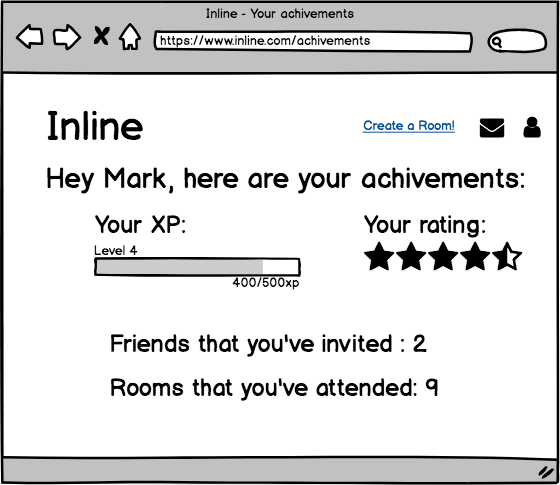
\includegraphics[width=\textwidth]{./Mockup/achivements.png}
		\end{minipage}
		\hfill
		\begin{minipage}[b]{0.45\textwidth}
			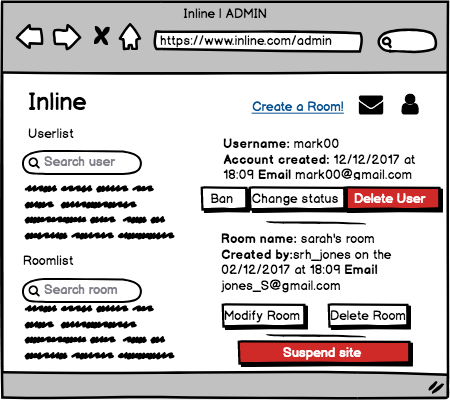
\includegraphics[width=\textwidth]{./Mockup/admin.png}
		\end{minipage}
	\end{figure}

	\begin{figure}[H]
		\centering
		\begin{minipage}[b]{0.45\textwidth}
			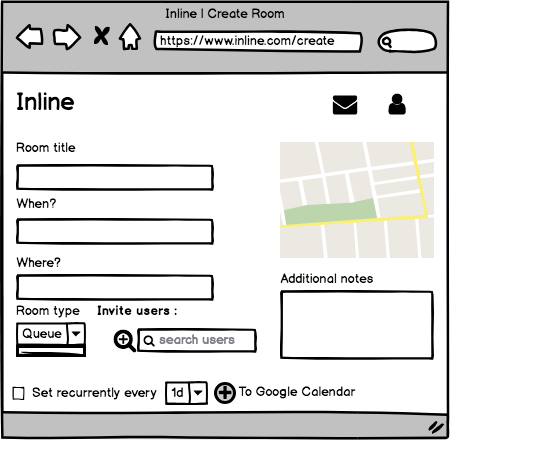
\includegraphics[width=\textwidth]{./Mockup/Createevent.png}
		\end{minipage}
		\hfill
		\begin{minipage}[b]{0.45\textwidth}
			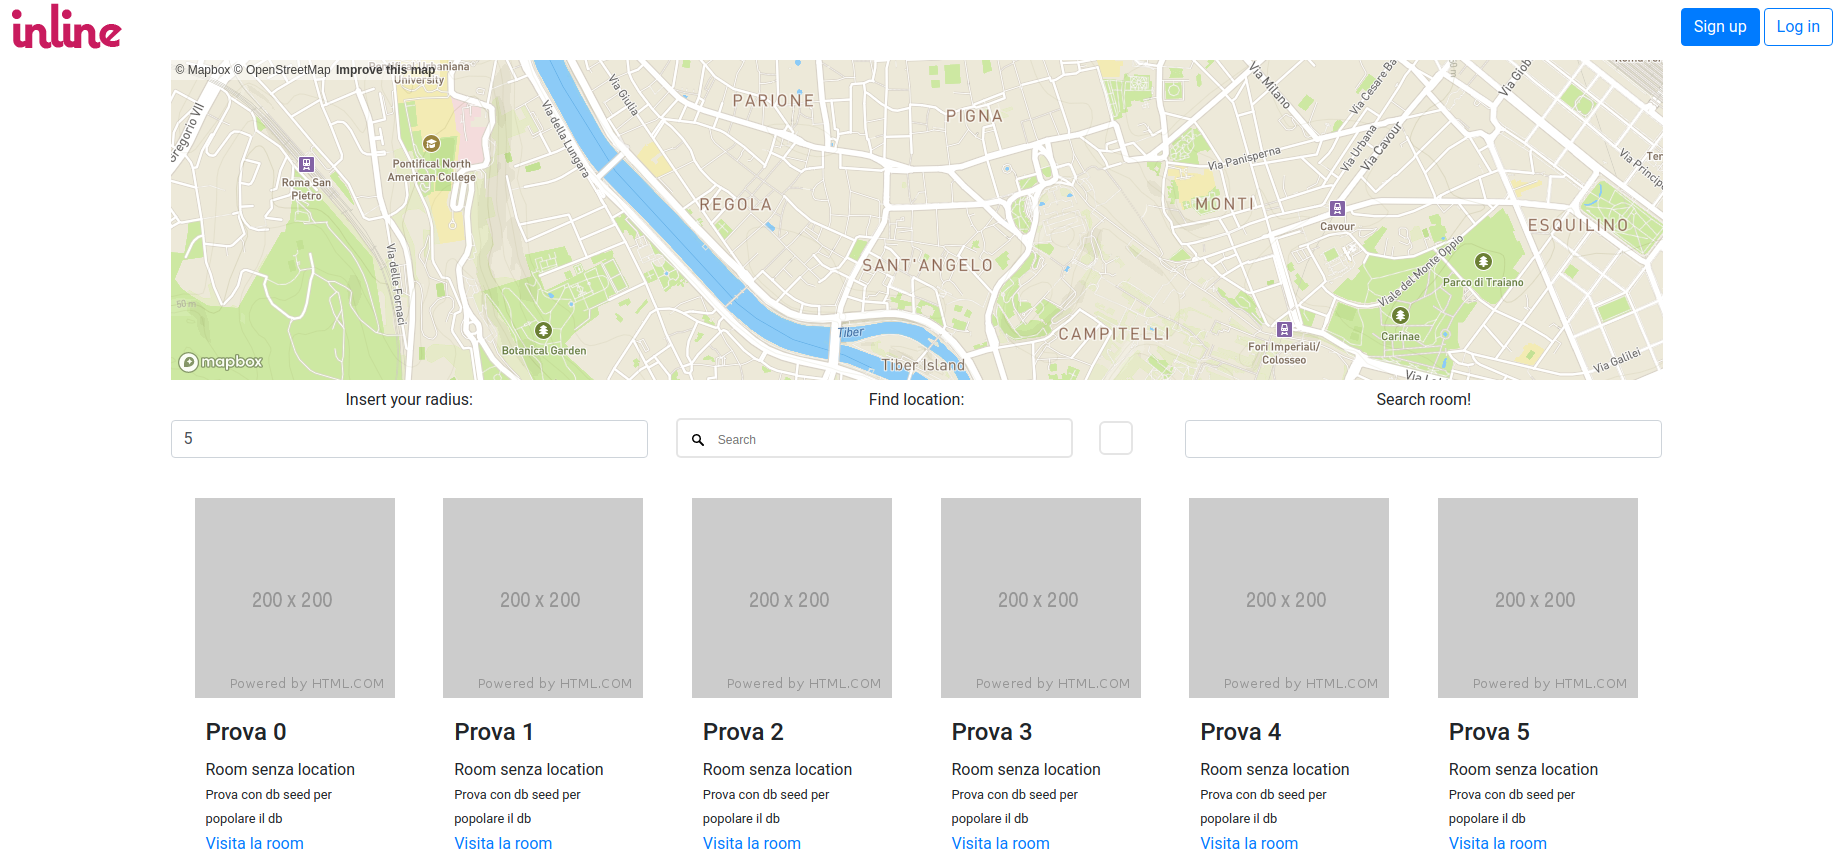
\includegraphics[width=\textwidth]{./Mockup/Dashboard.png}
		\end{minipage}
	\end{figure}

	\begin{figure}[H]
		\centering
		\begin{minipage}[b]{0.45\textwidth}
			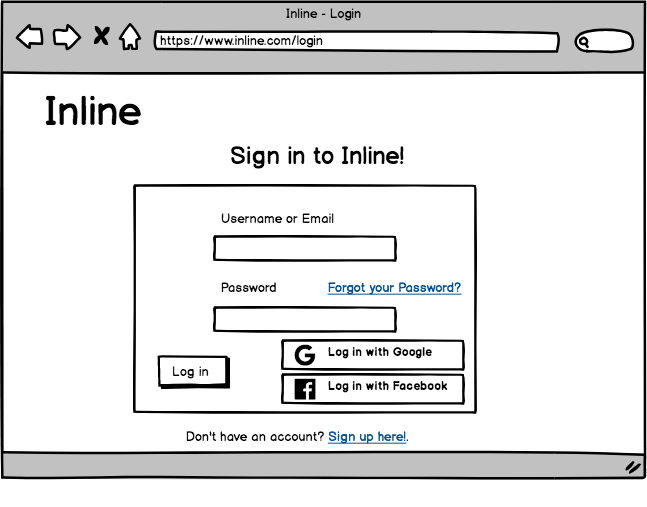
\includegraphics[width=\textwidth]{./Mockup/login.png}
		\end{minipage}
		\hfill
		\begin{minipage}[b]{0.45\textwidth}
			\includegraphics[width=\textwidth]{./Mockup/Modify.png}
		\end{minipage}
	\end{figure}

	\begin{figure}[H]
		\centering
		\begin{minipage}[b]{0.45\textwidth}
			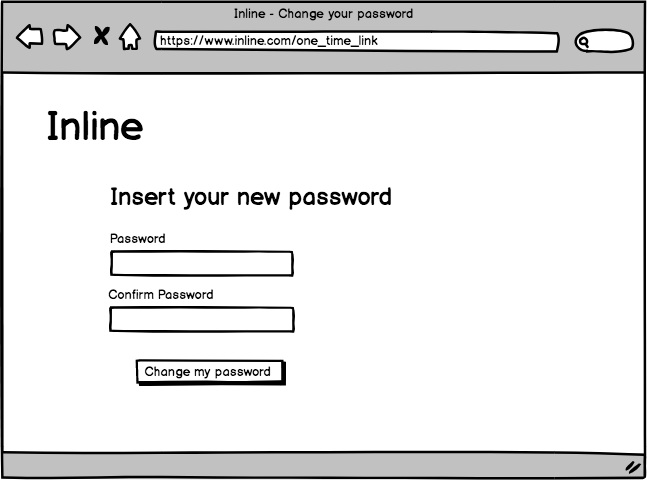
\includegraphics[width=\textwidth]{./Mockup/password.png}
		\end{minipage}
		\hfill
		\begin{minipage}[b]{0.45\textwidth}
			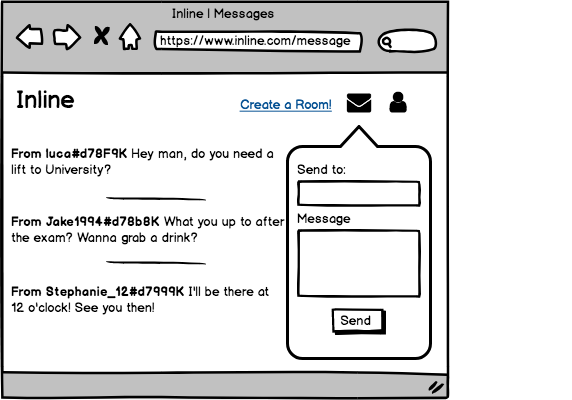
\includegraphics[width=\textwidth]{./Mockup/pms.png}
		\end{minipage}
	\end{figure}

	\begin{figure}[H]
		\centering
		\begin{minipage}[b]{0.45\textwidth}
			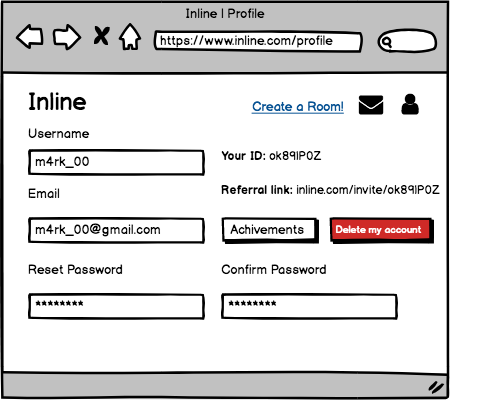
\includegraphics[width=\textwidth]{./Mockup/profile.png}
		\end{minipage}
		\hfill
		\begin{minipage}[b]{0.45\textwidth}
			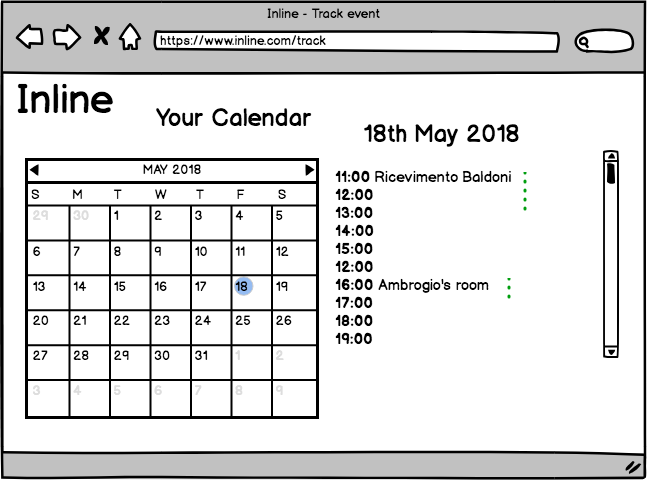
\includegraphics[width=\textwidth]{./Mockup/track.png}
		\end{minipage}
	\end{figure}

	\begin{figure}[H]
		\centering
		\begin{minipage}[b]{0.45\textwidth}
			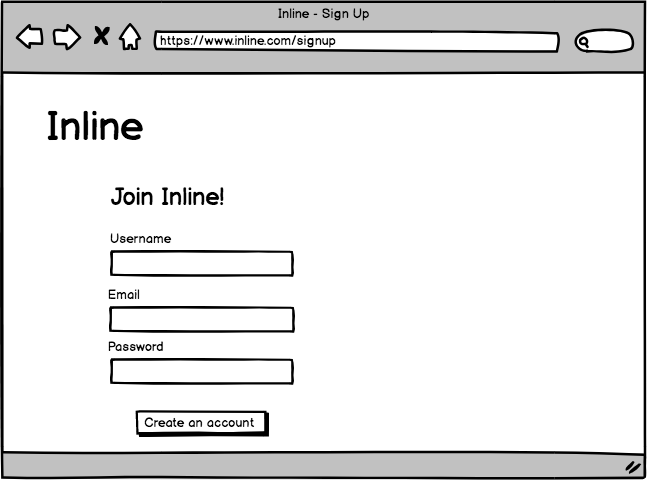
\includegraphics[width=\textwidth]{./Mockup/signup.png}
		\end{minipage}
		\hfill
		\begin{minipage}[b]{0.45\textwidth}
			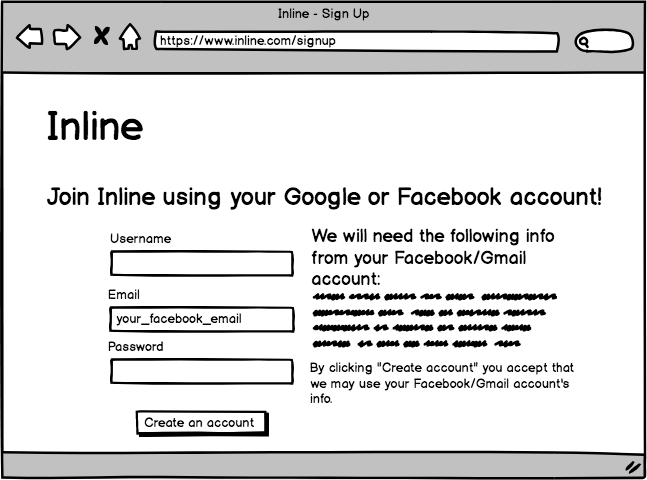
\includegraphics[width=\textwidth]{./Mockup/oauth.png}
		\end{minipage}
	\end{figure}

	\begin{figure}[H]
		\centering
		\begin{minipage}[b]{0.85\textwidth}
			\includegraphics[width=\textwidth]{./Mockup/room.png}
		\end{minipage}
	\end{figure}
